\chapter{Datasets}
\label{datasets_chapter}

The experiments conducted in this thesis use the same datasets as those utilized in the previous work by Jan Flajžík \cite{flajzik_classification_2024}. Three of the datasets contain English-language texts, while one dataset consists of Czech-language texts.

Some preprocessing techniques from the original implementation, such as noise reduction, stemming, and lemmatization, were reused and adapted for the transformer-based pipeline used in this work. At the same time, additional tokenization approaches suitable for transformer architectures were introduced.

For all datasets used in this thesis, the target labels follow the same convention:
- label \texttt{0} represents fake (unreliable news),
- label \texttt{1} represents reliable news.


\section{ReCOVery Dataset}

The ReCOVery dataset was created following the COVID-19 pandemic and is intended for research focused on the credibility of COVID-19-related news articles. The dataset contains English-language articles discussing both the pandemic itself and its political and social consequences.

The original ReCOVery dataset is multimodal. However, in the previous work on which this thesis builds, only textual information was used. The same approach is adopted in this thesis. All columns except the article title and textual content were removed, and the remaining textual information was processed as a single input sequence.

The ReCOVery dataset is notably imbalanced, as illustrated in Figure \ref{fig:recovery_labels_distribution}. Although this imbalance was acknowledged in the previous work, no balancing techniques were applied. The same approach is followed in this thesis, and the imbalance should therefore be considered when interpreting the experimental results \cite{flajzik_classification_2024}.

\begin{figure}[!htbp]
    \centering
    
\includegraphics[width=\linewidth]{assets/recovery/label_distribution.png}
    \caption{Distribution of labels in the ReCOVery dataset}
    \label{fig:recovery_labels_distribution}
\end{figure}

\FloatBarrier

Since this thesis utilizes transformer-based architectures, token length becomes an important factor during training and evaluation. Transformer models operate with a fixed input length, meaning that articles exceeding the selected token limit must be truncated. Consequently, parts of longer articles are discarded and are not considered during feature extraction or prediction.

The token length distribution for the ReCOVery dataset using the BERT tokenizer is shown in Figure \ref{fig:recovery_bert_token_length_distr}. The figure presents a histogram of article lengths measured in tokens together with several selected input length limits. Larger token windows allow the model to process more information from each article, but they also significantly increase computational requirements and training time.

In this work, the maximum sequence length was limited to 512 tokens. Although larger context windows such as 1024 tokens were considered, their computational cost was too high for the available computational resources. A similar simplification strategy was also applied in \cite{flajzik_classification_2024} in order to keep the experiments computationally feasible.

\begin{figure}[!htbp]
    \centering
    
\includegraphics[width=\linewidth]{assets/recovery/bert_token_length_distribution.png}
    \caption{Distribution of token lengths in the ReCOVery dataset using the BERT tokenizer}
    \label{fig:recovery_bert_token_length_distr}
\end{figure}

\FloatBarrier

The presented label distribution and token length analysis provide important information about the characteristics of the dataset. Compared to the other datasets used in this thesis, the ReCOVery dataset contains relatively long articles, in some cases exceeding 5000 tokens. A sequence length of 512 tokens therefore covers less than half of articles.

As a result, the transformer models used in this work process only partial information from longer texts, typically focusing on the beginning of the article. This represents a significant limitation of the current experimental setup and may negatively affect the models’ ability to detect disinformation patterns appearing later in the text.


\section{ISOT Dataset}

\begin{markdown}


The ISOT Fake News Dataset is a widely used benchmark dataset for fake news classification tasks. It contains more than 44,000 articles, where reliable news articles were obtained from the Reuters news agency, while fake news articles were collected from unreliable sources and verified using fact-checking resources such as Politifact and Wikipedia . The dataset primarily focuses on political news published during 2016 and 2017, with a significant emphasis on topics related to former United States President Donald Trump and his policies \cite{flajzik_classification_2024}.

In the previous work by Jan Flajžík \cite{flajzik_classification_2024}, several preprocessing and simplification steps were applied to the original dataset:

- the dataset was reduced to 10,000 articles in order to decrease the size difference between ISOT and the remaining datasets,
- articles published in 2016 were removed,
- the \texttt{subject} attribute was excluded because the categories of fake and reliable news did not overlap, making the classification task artificially simple,
- the resulting dataset remained relatively balanced, containing approximately 53\% reliable news and 47\% fake news.

The label distribution of the resulting dataset is shown in Figure \ref{fig:isot_labels_distribution}, while the token length distribution using the BERT tokenizer is shown in Figure \ref{fig:isot_bert_token_length_distr}.

Compared to the ReCOVery dataset, the ISOT dataset contains substantially more articles, while the average article length is generally shorter. As a result, the selected maximum sequence length of 512 tokens covers a considerably larger portion of the dataset, allowing transformer models to process a greater amount of information from each article.

\end{markdown}

\begin{figure}[!htbp]
    \centering
    
\includegraphics[width=\linewidth]{assets/isot/label_distribution.png}
    \caption{Distribution of labels in the ISOT dataset}
    \label{fig:isot_labels_distribution}
\end{figure}

\begin{figure}[!htbp]
    \centering
    
\includegraphics[width=\linewidth]{assets/isot/bert_token_length_distribution.png}
    \caption{Distribution of token lengths in the ISOT dataset using the BERT tokenizer}
    \label{fig:isot_bert_token_length_distr}
\end{figure}

\FloatBarrier

\section{EUvsDisinfo Dataset}

\begin{markdown}

The EUvsDisinfo dataset used in the previous work by Jan Flajžík \cite{flajzik_classification_2024} was constructed using data from the EUvsDisinfo project operated by the European External Action Service’s East StratCom Task Force. The initiative was established in 2015 with the goal of monitoring and documenting disinformation campaigns associated with the Russian Federation.

Several modifications were applied in order to create a suitable dataset for binary fake news classification experiments \cite{flajzik_classification_2024}:

- instead of full articles, short English summaries describing disinformation cases were used,
- reliable news summaries were collected from \textit{The Guardian} to create a balanced counterpart dataset,
- the resulting dataset contains 2,139 text samples with an almost balanced distribution between reliable and unreliable news,
- because the dataset consists of summaries rather than full articles, the length of each sample is relatively short.

According to \cite{flajzik_classification_2024}, shorter textual inputs appeared to be more suitable for certain neural architectures such as LSTM models, which achieved better results on this dataset than on datasets containing longer articles. The use of summaries may also better reflect modern online media consumption, where users often interact primarily with short-form textual content.

The label distribution of the dataset is shown in Figure \ref{fig:euvsdisinfo_labels_distribution}, while the token length distribution obtained using the BERT tokenizer is shown in Figure \ref{fig:euvsdisinfo_bert_token_length_distr}.

Compared to the previously discussed datasets, the EUvsDisinfo dataset contains significantly shorter text samples. As a result, the selected transformer input window of 512 tokens is sufficient to process the complete text for all samples without truncation.

\end{markdown}

\begin{figure}[!htbp]
    \centering
    
\includegraphics[width=\linewidth]{assets/euvsdisinfo/label_distribution.png}
    \caption{Distribution of labels in the EUvsDisinfo dataset}
    \label{fig:euvsdisinfo_labels_distribution}
\end{figure}

\begin{figure}[!htbp]
    \centering
    
\includegraphics[width=\linewidth]{assets/euvsdisinfo/bert_token_length_distribution.png}
    \caption{Distribution of token lengths in the EUvsDisinfo dataset using the BERT tokenizer}
    \label{fig:euvsdisinfo_bert_token_length_distr}
\end{figure}

\FloatBarrier

\begin{markdown}

The token length analysis shows that the text samples in this dataset are relatively short. Since the vast majority of samples remain below the selected limit of 512 tokens, the transformer models are able to process the complete summaries without truncation. Consequently, the models can utilize the full textual information available in the dataset during both training and evaluation.

\end{markdown}

\section{Czech Dataset}

\begin{markdown}

The Czech dataset used in \cite{flajzik_classification_2024} was created specifically for fake news detection experiments focused on the Czech media environment. The dataset primarily targets disinformation distributed through chain emails, which represent a common channel for spreading misleading information in the Czech Republic.

The dataset consists of both fake and reliable textual sources:

- 405 fake news texts were obtained from the Eldariel database maintained by the citizen initiative \textit{Čeští elfové},
- approximately 30\% of the fake content consists directly of chain email texts, while the remaining samples contain articles referenced within those emails,
- reliable news articles were collected from the Czech public television news portal \textit{ČT24},
- the resulting dataset contains 995 text samples with an approximate ratio of 59\% reliable news and 41\% fake news.

The collected texts focus primarily on international political topics related to Russia and Ukraine during 2022 and the beginning of 2023. During dataset preparation, entries containing only images or links without sufficient textual content were removed.

Because Czech natural language processing requires language-specific preprocessing tools, the original implementation used several Czech-oriented resources and libraries, including Czech stemming tools, multilingual lemmatization libraries, and pretrained Czech language embeddings.

\end{markdown}

\begin{figure}[!htbp]
    \centering
    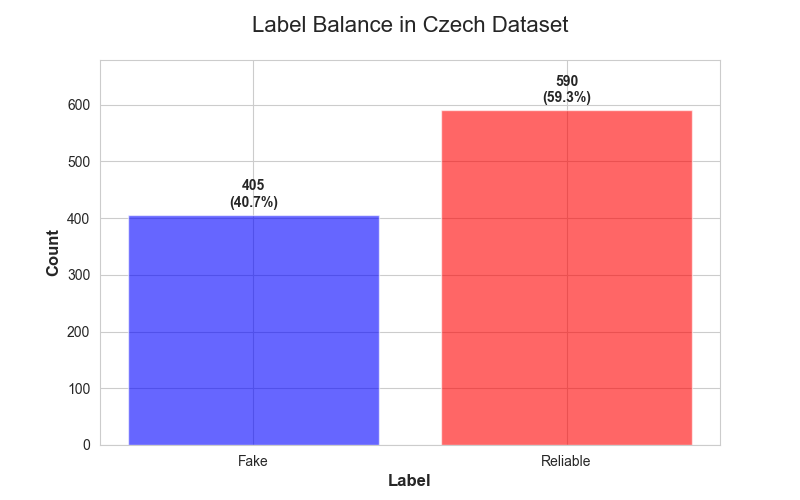
\includegraphics[width=\linewidth]{assets/cz_dataset/label_distribution.png}
    \caption{Distribution of labels in the Czech dataset}
    \label{fig:cz_dataset_labels_distribution}
\end{figure}

\begin{figure}[!htbp]
    \centering
    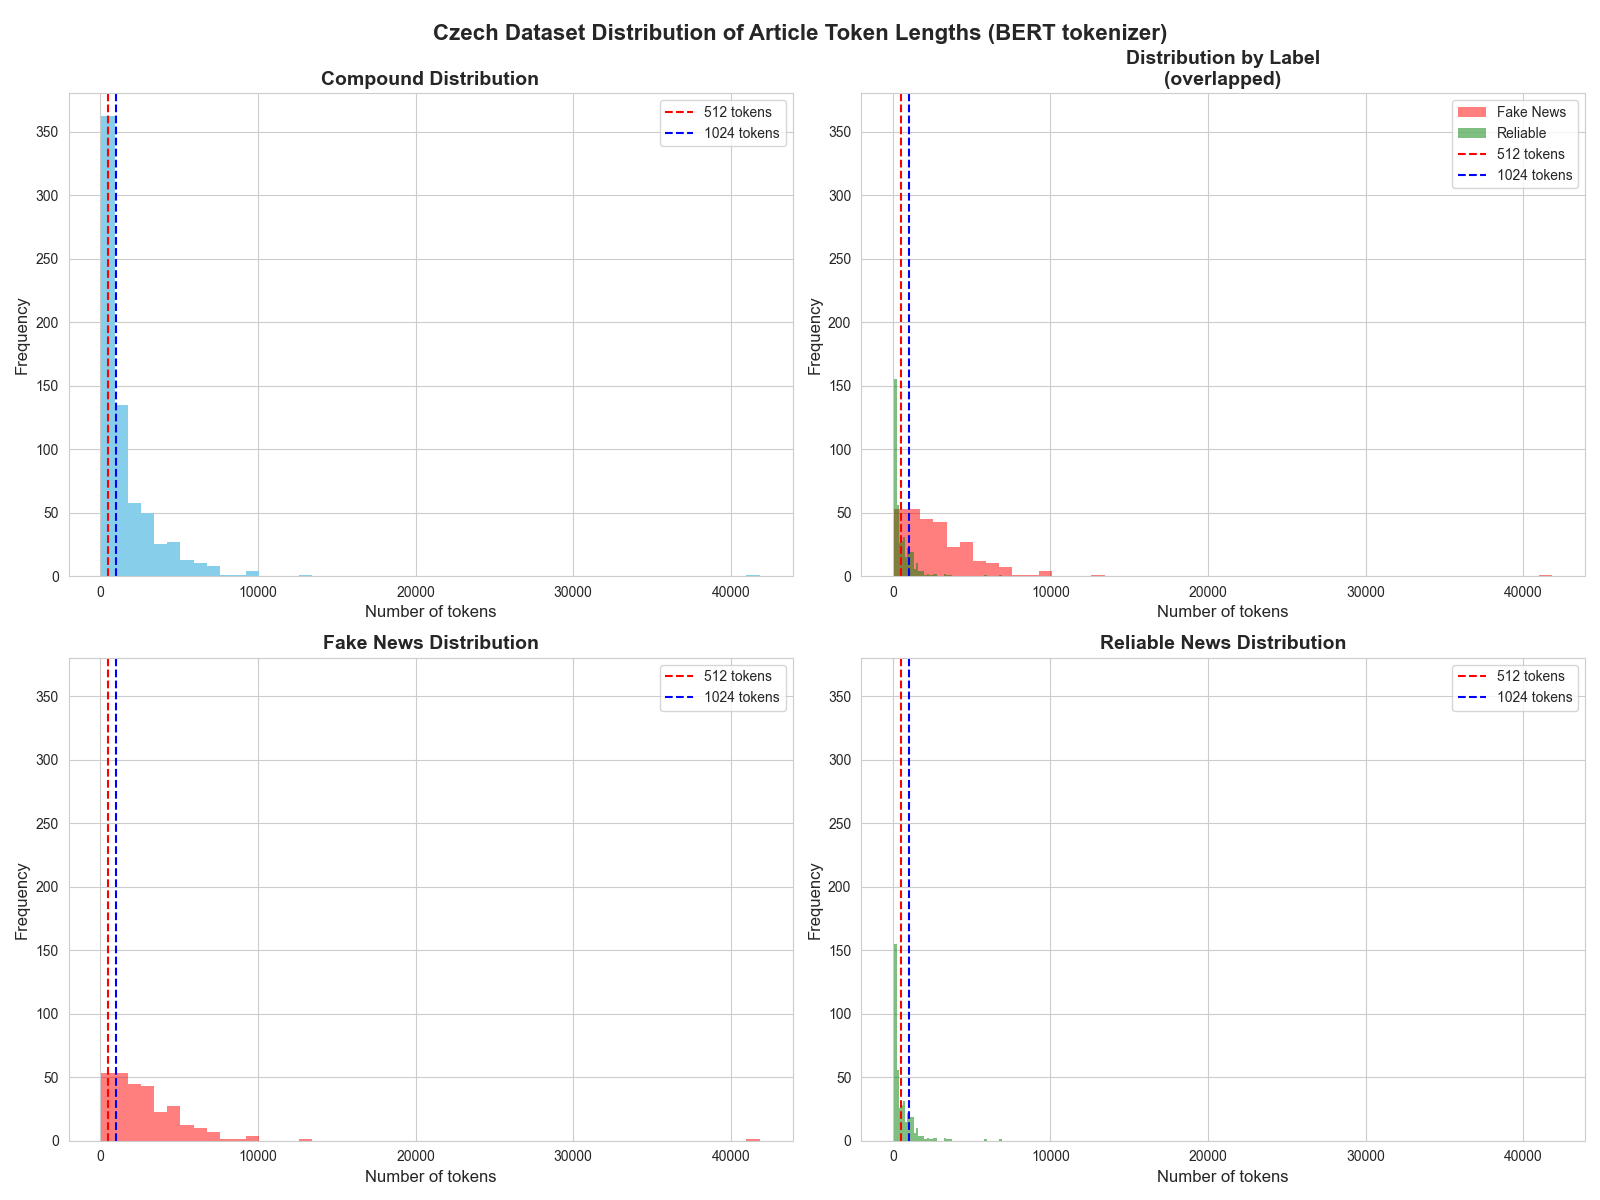
\includegraphics[width=\linewidth]{assets/cz_dataset/bert_token_length_distribution.png}
    \caption{Distribution of token lengths in the Czech dataset using the BERT tokenizer}
    \label{fig:cz_dataset_bert_token_length_distr}
\end{figure}

\FloatBarrier

\section{Summary}

The dataset analysis highlights one of the main limitations of the experimental setup used in this thesis. Although transformer-based architectures are capable of processing complex textual information, the fixed input length restriction prevents the models from utilizing the full content of many long articles.

A more suitable approach could involve splitting longer articles into multiple segments and adapting the training process accordingly so that the entire text can be processed. Such an approach would likely provide richer contextual information to the models, although it would also increase computational requirements and implementation complexity.

The experiments conducted in this thesis therefore primarily evaluate how transformer-based architectures perform under constrained conditions, where only partial textual information is available for many samples. This limitation may lead the models to rely on more superficial textual patterns, potentially reducing generalization performance and increasing the risk of overfitting.



